\documentclass[margin,line,a4paper]{resume}

\usepackage[utf8]{inputenc} %utf8
\usepackage[english,danish]{babel}
%\usepackage[T1]{fontenc} %Gives font a gray look on screen :-(
\usepackage{graphicx}
\usepackage{graphicx,wrapfig}
%\usepackage{url}
\usepackage[colorlinks=true, a4paper=true, pdfstartview=FitV,linkcolor=blue, citecolor=blue, urlcolor=blue]{hyperref}
\pdfcompresslevel=9

\usepackage{lastpage}
\usepackage{fancyhdr}
%\usepackage[page]{totalcount}

%\usepackage{zref-user,zref-lastpage}
% \usepackage{everyshi}
% \usepackage{keyval}
% \usepackage{totpages}
\pagestyle{fancy}
\fancyhf{}
\renewcommand{\headrulewidth}{0pt}
\rfoot{Page \thepage~of \pageref*{LastPage}}

\begin{document}
{\sc \Large Curriculum Vitae -- Torben Green}
\begin{resume}
    \vspace{0.5cm}
    \begin{wrapfigure}{R}{0.6\textwidth}
      \vspace{-1cm}
      \begin{center}
        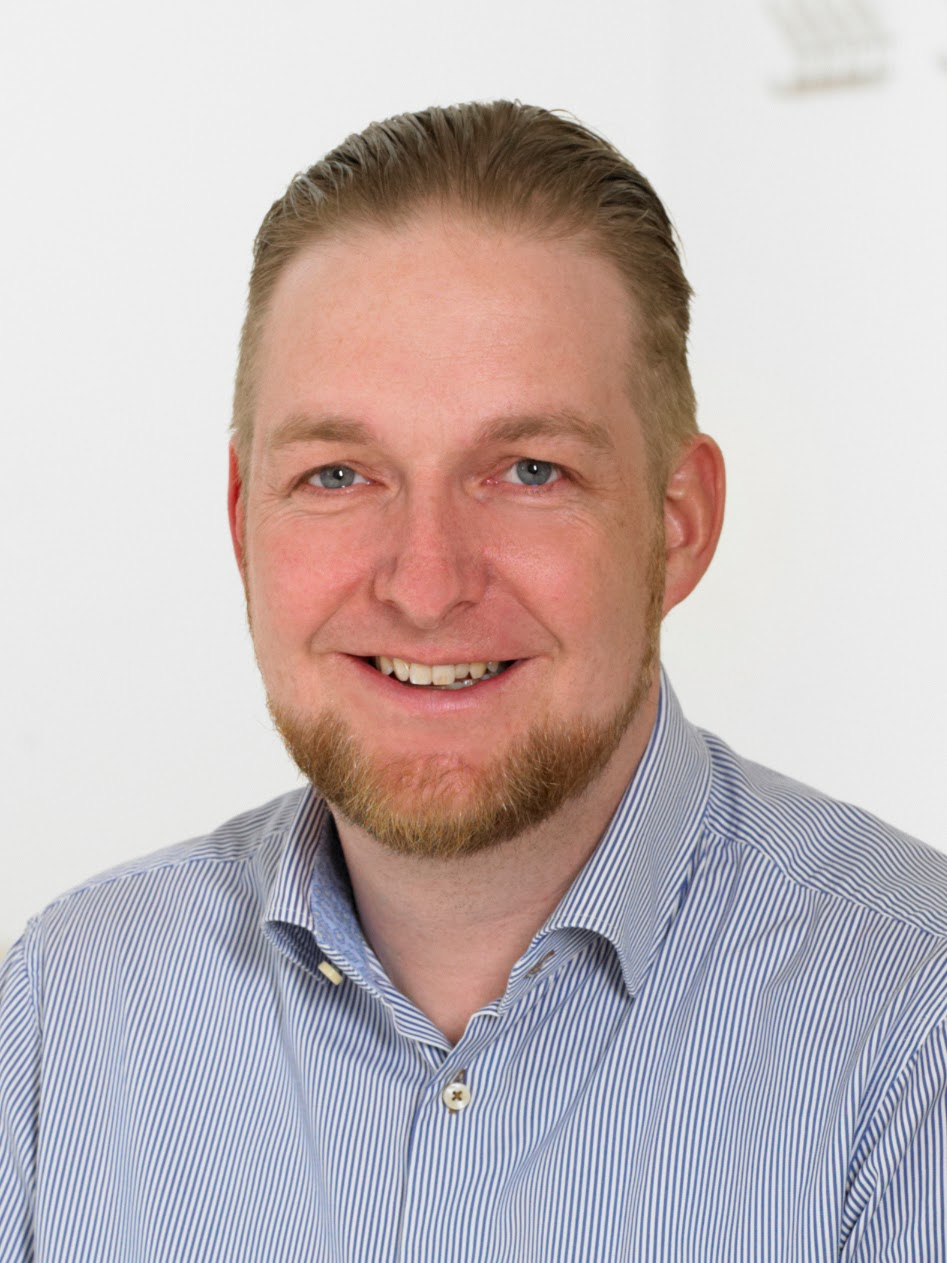
\includegraphics[width=0.4\textwidth]{TOGhrweb}
        %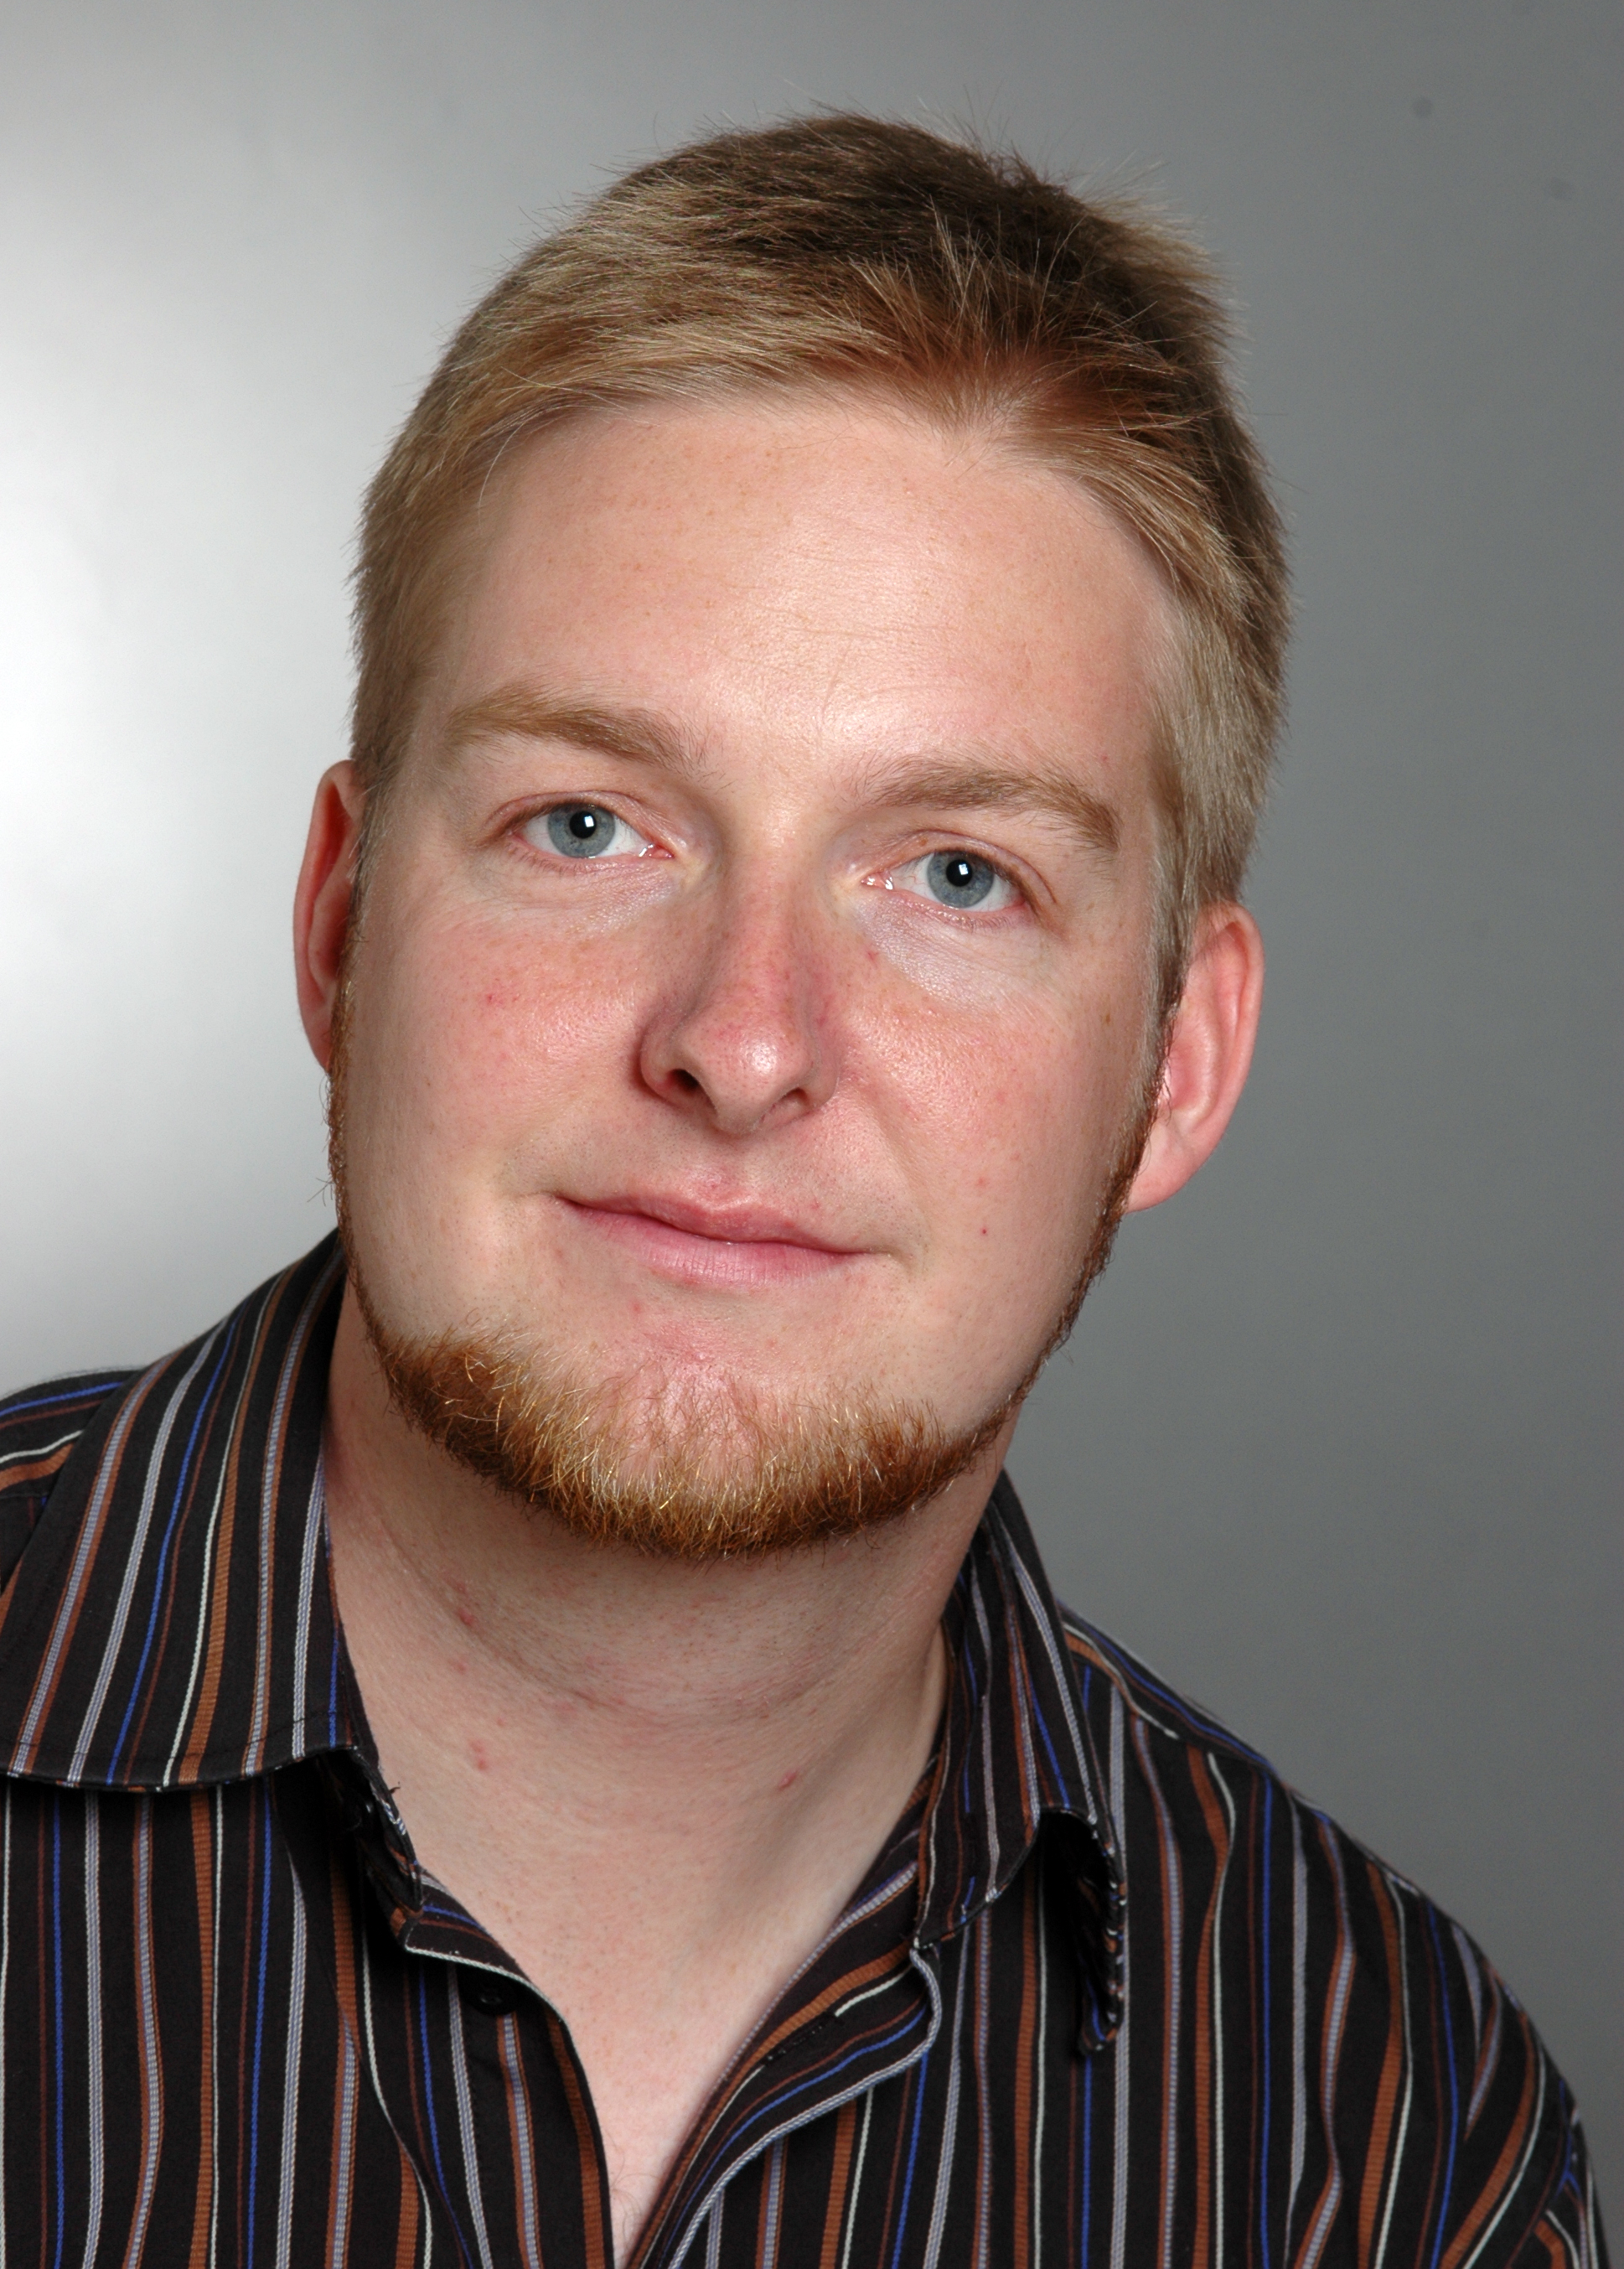
\includegraphics[width=0.4\textwidth]{me}
      \end{center}
      \vspace{-1cm}
    \end{wrapfigure}

    \section{\mysidestyle Personal\\Information}%\vspace{2mm}
    Torben Green \\
    Tel: +45 72202427 \\
    Birthday: January 31$^{\rm st}$ 1982\\
    \href{mailto:tog@teknologisk.dk}{tog@teknologisk.dk}
    %\href{mailto:torben.green@danfoss.com}{torben.green@danfoss.com} \\
    %\href{http://dk.linkedin.com/in/torbengreen}{http://dk.linkedin.com/in/torbengreen}\\
    %\href{https://twitter.com/#!/torben_g}{Twitter: @torben\_g} 
%I was born in Aabenraa on January the 31$^{\rm st}$ of 1982, where I have lived for the majority of my life. I am currently working for Danfoss A/S as a research engineer. Since 2011 my research has been focused on Smart Grid or Smart Energy integration of refrigeration systems. 

Structured and customer focued R\&D engineer with an analytical approach toward problem solving. Interest include, refrigeration and heat pump systems, energy optimization, performance assesment of dynamic systems, business analysis and value proposition. Work experience include, development of control algorithms, project management of innovation projects, and creating value propositions and business analysis for novel business ideas.

%My approach toward research is very business oriented. I am always evaluating the risk of a research project against the potential outcome. The ability to complete a research project depends on the ability choose the right project to pursue. 
    
\section{\mysidestyle Job Experiences}\vspace{1mm}
\begin{description}
\item[2016 April$\rightarrow$ Present] Employed as consultant at Danish Technological Institute, Center for Refrigeration and Heat Pump Technology.

   \item[2014 April$\rightarrow$ Present] Registered as censor for the engineering education within the field of electronics at \href{https://www.censornet.dk/welcome.htm}{censornet.dk}
     \begin{itemize}
     \item Worked as censor on Master level at both Technical University of Denmark and Aalborg University.
     \item Worked as censor on Bachelor level at Aalborg University in Aalborg and in Esbjerg.
     \end{itemize}
    
    \item[2012 April$\rightarrow$ 2016 March] Employed as Research Engineer at Danfoss A/S, Refrigeration \& Air Conditioning. Assignments include:
      \begin{itemize}
      \item Developing, implementing and testing advanced control algorithms for supermarket refrigeration systems.
      \item Participating in a number public funded research projects within the area of energy optimization, Smart Grid and Smart Energy. Techical lead from Danfoss in the iPower, ELIS and ZeroGi projects.
      \item Promoting projects internally and externally.
      \item Collaboration with costumers, universities and other external partners on projects. 
      \item Project management of innovation projects.
      \item Creating business cases and value propositions.
      \item Protection of IPR. Filed 5 patent applications.
      \end{itemize}

    \item[2008 December$\rightarrow$ 2012 March] Industrial Ph.D. student at Danfoss and the Technical University of Denmark. Assignments during my Ph.D.:
      \begin{itemize}
      \item Dynamic modeling of supermarket refrigeration systems.
      \item Describing global performance of a complicated dynamic system with a distributed control system.
      \item Active and passive fault detection and diagnosis.
      \item Simulating proposed algorithms based on data from real supermarkets.
      \item Presenting research results at international conferences. 
      \end{itemize}

    \item[2007 July$\rightarrow$ 2008 November] Employed as R \& D Engineer at Danfoss A/S, Refrigeration \& Air Conditioning. My main focus was development of control and adaptation algorithms for a new valve for refrigerant injection for the residential air conditioning market. In addition, my work included analysis of the operational performance of the distributed control architecture for supermarket refrigeration systems.
      Assignments included:
      \begin{itemize}
      \item Developing control algorithms for a new type of electronic expansion valve, the Danfoss EcoFlow valve.
      \item Running tests of control algorithms in refrigeration laboratory.
      \item Running tests of control algorithms at a customer site.
      \item Analyzing performance issues of supermarket refrigeration systems.
      \end{itemize}

\end{description} 

\section{\mysidestyle Education} 

    \textbf{Ph.D.} (2008 December - 2012 September). Thesis title: \textit{Performance assessment and active system monitoring for refrigeration systems}. 

    \textbf{Master of Science in Engineering, Control engineering}
    (2002-2007). Specialization in Intelligent Autonomous systems. Working on projects related to refrigeration from the 8$^{\rm th}$ to the 10$^{\rm th}$ semester.
    
    \textbf{Military Service} (2001-2002) Basic military training at Dronningens Artilleriregiment in Skive.

    \textbf{HTX Aabenraa} (1998-2001) High school.  Higher technical exam, (HTX), at EUC syd Aabenraa.


\section{\mysidestyle Programming Languages}

Fluent in \textbf{C}, \textbf{Python} and \textbf{Matlab}. Proficient in \textbf{Make}, \textbf{Bash} and \textbf{Modelica}

\section{\mysidestyle Languages}

\textbf{Danish}: Mother tongue. \textbf{English}: Fluent. \textbf{German}: High-school level.

% \section{\mysidestyle Additional Information}

% I am married with Lotte, who is a school teacher, and we have two boys ages 5 and 7. In my spare time I like to exercise and I am also active in Det Danske Spejderkorps as scout leader for children ages 12-16.


\section{\mysidestyle Patent \\Applications}

Jan Prins, Frede Schmidt, Torben Green, \textit{Match Load to Capacity}, PA15445EP01.

Torben Funder-Kristensen, Allan Slot, Torben Green, \textit{Energy management in refrigeration systems}, PA15500EP02.

Torben Green, Rasmus Pedersen, John Schwensen, Jakob Stoustrup, Benjamin Biegel, \textit{Temperature estimation of foodstuff}, PA15868WO01.

Plus two applications waiting to be published.

\section{\mysidestyle Selected Publications}

Lisa Buth Rasmussen, Peder Bacher, Henrik Madsen, Henrik Aalborg Nielsen, Christian Heerup and Torben Green \textit{Load forecasting of supermarket refrigeration}, Published in Applied Energy Volume 163, 1 February 2016, Pages 32–40, \href{https://doi.org/10.1016/j.apenergy.2015.10.046}{https://doi.org/10.1016/j.apenergy.2015.10.046}.

Torben Green, Roozbeh Izadi-Zamanabadi, Roozbeh Razavi-Far and Henrik Niemann. \textit{Plant-wide Dynamic and Static Optimisation of Supermarket Refrigeration Systems}, Published in the International Journal of Refrigeration, Available online 20 August 2013, \href{http://dx.doi.org/10.1016/j.ijrefrig.2013.08.011}{http://dx.doi.org/10.1016/j.ijrefrig.2013.08.011}.

Torben Green, Roozbeh Razavi-Far, Roozbeh Izadi-Zamanabadi and Henrik Niemann. \textit{Plant-wide performance optimisation -- The refrigeration system case}, In the proceedings of the 2012 IEEE Multi-Conference on Systems and Control, pp. $208-213$, Dubrovnik 2012.

Torben Green, Michel Kinnart, Roozbeh Razavi-Far, Roozbeh Izadi-Zamanabadi and Henrik Niemann. \textit{Optimising performance in steady state for a supermarket refrigeration system}, In the proceedings of the 20th IEEE Mediterranean Conference on Control and Automation, pp. $1061-1066$, Barcelona 2012.

Torben Green, Roozben Izadi-Zamanabadi and Henrik Niemann, \textit{Design of Excitation Signal for Active System Monitoring in a Performance Assessment Setup}, In the proceedings of the 9th European Workshop on Advanced Control and Diagnosis, Budapest 2011.

Torben Green, Henrik Niemann and Roozbeh Izadi-Zamanabadi, \textit{Performance improvement clarification for refrigeration system using active system monitoring}, In the proceedings of the 18$^{th}$ IFAC World Congress, pp. $2845-2850$, Milan 2011. 

Torben Green, Roozbeh Izadi-Zamanabadi and Henrik Niemann, \textit{On the choice of performance assessment criteria and their impact on the overall system performance -- The refrigeration system case study}, In the proceedings of the First IEEE Conference on Control and Fault-Tolerant Systems (SysTol'10), pp. $624-629$, Nice 2010.


Liang Chen,  Torben Green, Roozbeh Izadi-Zamanabadi and Lars F. S. Larsen,
\textit{Early Measure of Synchronization Operations in Supermarket Refrigeration Systems}, In  the proceedings of Sims50, Fredericia 2009.

Liang Chen,  Torben Green, Lars F. S. Larsen, Rafael Wisniewski and Roozbeh Izadi-Zamanabadi, \textit{Performance Monitoring in Supermarket Refrigeration Systems - Synchronization of Refrigerated Display Cases}, In the proceedings of IFAC Symposium on Advanced Control of Chemical Processes Symposium, Istanbul 2009.

\end{resume}
\end{document}
